% Documenting the issue that there is a yield penalty on monoculture that is less than expected
% Look at three-year rotations as well and soybeans, look at model for covariates

% Runoff and waterways effect of monoculture, is it associated with greater runoff?

\documentclass[notes, 11pt, aspectratio=169]{beamer}
\usepackage{pgfpages}
% These slides also contain speaker notes. You can print just the slides,
% just the notes, or both, depending on the setting below. Comment out the want
% you want.
\setbeameroption{hide notes} % Only slide
\setbeamertemplate{caption}[numbered]
%\setbeameroption{show only notes} % Only notes
%\setbeameroption{show notes on second screen=right} % Both
\setbeamertemplate{footline}[page number]

\usepackage{helvet}
\usepackage[default]{lato}
\usepackage{array}
\usepackage{tikz}
\usepackage{verbatim}
\usepackage{natbib}
\bibliographystyle{apalike}
\usepackage[affil-it]{authblk}
\tikzset{>=latex} % for LaTeX arrow head
\usepackage{pgfplots} % for the axis environment
\pgfplotsset{compat=1.18}
\usepackage{xcolor}
\usepackage{adjustbox}
\usepackage[outline]{contour} % halo around text
\setbeamertemplate{note page}{\pagecolor{yellow!5}\insertnote}
\contourlength{1.2pt}
\usepackage{amsmath}
\usepackage{newpxtext}
\usepackage[osf]{mathpazo}
\usepackage{hyperref}
\usepackage[pdf]{pstricks}
\usepackage{epstopdf}
\epstopdfsetup{update}
\usepackage{multimedia}
\usepackage{multirow}
\usepackage{dcolumn}
\usepackage{animate}
\usepackage{bbm}
\usepackage{booktabs}
\usepackage{blindtext}

\newcolumntype{d}[0]{D{.}{.}{5}}

\usepackage{changepage}
\usepackage{appendixnumberbeamer}
\newcommand{\beginbackup}{
   \newcounter{framenumbervorappendix}
   \setcounter{framenumbervorappendix}{\value{framenumber}}
   \setbeamertemplate{footline}
   {
     \leavevmode%
     \hline
     box{%
       \begin{beamercolorbox}[wd=\paperwidth,ht=2.25ex,dp=1ex,right]{footlinecolor}%
%         \insertframenumber  \hspace*{2ex} 
       \end{beamercolorbox}}%
     \vskip0pt%
   }
 }
\newcommand{\backupend}{
   \addtocounter{framenumbervorappendix}{-\value{framenumber}}
   \addtocounter{framenumber}{\value{framenumbervorappendix}} 
}


\usepackage{graphicx}
\usepackage[space]{grffile}
\usepackage{booktabs}

% These are my colors -- there are many like them, but these ones are mine.
\definecolor{blue}{RGB}{0,114,178}
\definecolor{red}{RGB}{213,94,0}
\definecolor{yellow}{RGB}{240,228,66}
\definecolor{green}{RGB}{0,158,115}

\hypersetup{
  colorlinks=false,
  linkbordercolor = {white},
  linkcolor = {blue}
}

%% I use a beige off white for my background
\definecolor{MyBackground}{RGB}{255,253,218}

%% Uncomment this if you want to change the background color to something else
%\setbeamercolor{background canvas}{bg=MyBackground}

%% Change the bg color to adjust your transition slide background color!
\newenvironment{transitionframe}{
	\setbeamercolor{background canvas}{bg=yellow}
	\begin{frame}}{
	\end{frame}
}

\setbeamercolor{frametitle}{fg=blue}
\setbeamercolor{title}{fg=black}
\setbeamertemplate{footline}[frame number]
\setbeamertemplate{navigation symbols}{} 
\setbeamertemplate{itemize items}{-}
\setbeamercolor{itemize item}{fg=blue}
\setbeamercolor{itemize subitem}{fg=blue}
\setbeamercolor{enumerate item}{fg=blue}
\setbeamercolor{enumerate subitem}{fg=blue}
\setbeamercolor{button}{bg=MyBackground,fg=blue,}


\setbeamercolor{section in toc}{fg=blue}
\setbeamercolor{subsection in toc}{fg=red}
\setbeamersize{text margin left=1em,text margin right=1em} 
\setbeamertemplate{footline}{\hspace*{.5cm}\scriptsize{\insertauthor
\hspace*{50pt} \hfill\insertframenumber\hspace*{-5cm}}}

\newenvironment{wideitemize}{\itemize\addtolength{\itemsep}{10pt}}{\enditemize}

\usepackage{environ}
\NewEnviron{videoframe}[1]{
  \begin{frame}
    \vspace{-8pt}
    \begin{columns}[onlytextwidth, T] % align columns
      \begin{column}{.58\textwidth}
        \begin{minipage}[t][\textheight][t]
          {\dimexpr\textwidth}
          \vspace{8pt}
          \hspace{4pt} {\Large \sc \textcolor{blue}{#1}}
          \vspace{8pt}
          
          \BODY
        \end{minipage}
      \end{column}%
      \hfill%
      \begin{column}{.42\textwidth}
        \colorbox{green!20}{\begin{minipage}[t][1.2\textheight][t]
            {\dimexpr\textwidth}
            Face goes here
          \end{minipage}}
      \end{column}%
    \end{columns}
  \end{frame}
}

\title[]{Rainfall, Climate Shifts, and Impacts on Forage Production Risks: Implications for Indexed-Based Insurance Rating}
\author[VEF]{}
\institute[UARK]{\small{\begin{tabular}{cc}
			Lawson Connor & Victor Funes-Leal & Eunchun Park\\
			\multicolumn{3}{c}{\small Department of Agricultural Economics and Agribusiness}\\ 
			\multicolumn{3}{c}{\small University of Arkansas}\\
\end{tabular}}}
 
\makeatletter

\begin{document}

% Title Slide
 
\begin{frame}
	\maketitle
	\centering 
\end{frame}

\begin{frame}{Outline}
\begin{wideitemize}
    \item \emph{Research Question}: How does crop rotation complexity affect harvest losses?
    \item \emph{Method}: We use linear fixed effects models to ascertain the magnitude of the relationship between these crop insurance losses and rotational complexity at a county level.
    \item \emph{Data}: County level (2005-2020) data on crop insurance losses data (RMA), Rotational complexity index (calculated from CDL), and weather variables (PRISM).
    \item \emph{Results}: The relationship between rotation complexity and crop losses depends critically on the timing of the latter: preventing planting losses is positively correlated with rotational complexity, but losses taking place close to harvest dates are negatively correlated with it.
\end{wideitemize}
\end{frame}

\begin{frame}{RMA Data}
    \begin{wideitemize}
        \item \emph{Loss data}: county-level information from crop losses (RMA), both Cause of loss (COL) and Summary of Business (SOB). We use data for: Yield Protection (YP), Revenue Protection (RP), and RP with Harvest Price Exclusion (RPHPE). 
        \item For preventing planting losses, we use the same \textit{stage codes} as \cite{won2024}. For post-emergence losses, we use all other stage codes. 
        \item We calculate two loss ratios:
        \begin{enumerate}
            \item Loss cost ratio (LCR): ratio of indemnities due to all causes of loss (from COL) over total liabilities (from SOB), similar to \cite{yu2024}.
            \item Loss acres ratio (LAR): ratio of total acres lost due to weather-related indemnities over total insured acres. 
        \end{enumerate}
    \end{wideitemize}
\end{frame}

\begin{frame}{RMA data and Cover crop adoption}
    \begin{wideitemize}
        \item Previous articles have studied the relationship between insurance losses and cover crop adoption \citep{aglasan2024, won2024}.
        \item They use county-level cover crop adoption percentage from OpTIS (Operational Tillage Information System), developed by Regrow Ag.
        \item OpTIS uses data from remotely sensed satellite data on conservation practices at the farm-field scale.
        \item These articles find a consistently negative relationship between cover crop adoption and losses.
    \end{wideitemize}
\end{frame} 

%\begin{frame}{Cover crop adoption}
%    \begin{figure}[H]
%    \centering
%    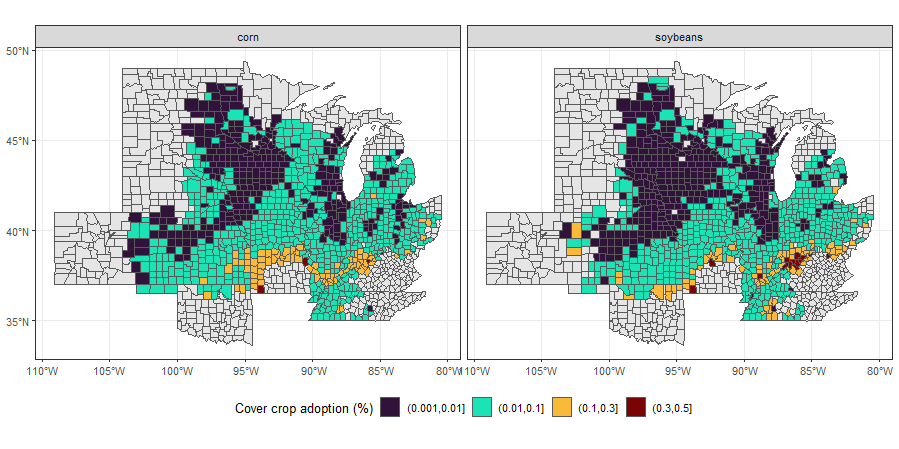
\includegraphics[scale = 0.5]{figures/cc_per.png}
%    \caption{Average cover crop adoption per county and crop (2005-2020)}
%    \label{fig:cc_per} 
%    \end{figure}
%\end{frame}

\begin{frame}{Rotation Complexity Index}
    \begin{wideitemize}
        \item The Rotational Complexity Index (RCI) from \cite{socolar2021}, is calculated based on crop sequences across six years at a field level.
        \item Let $T_{1}$ be the species turnover year-to-year on a given field, $T_{2}$, be the turnover every two years, and $T_{p}$ be the number of times a duplicate perennial appears in a field in two consecutive years (pseudo-turnover), then the RCI is:

        \begin{equation*}
            RCI = \sqrt{n\times\dfrac{T_{1}+T_{2}+T_{p}}{2}}
        \end{equation*}
        \item $n$ is the number of crops in the rotation. 
        \item RCI is a single number that can compare rotational complexity across any crop sequence.
        \item We use average harvested area-weighted RCI values per county/year throughout our analysis.
    \end{wideitemize}
\end{frame}

\begin{frame}{Rotation Complexity Index}
    \begin{wideitemize}
        \item \emph{Example 1}: six-year rotation of corn and soybeans (CSCSCS):
        \begin{itemize}
            \item \item $T_{1} = 5$, $T_{2} = 0$, $T_{p}=0$
            \item $RCI=\sqrt{2\times\dfrac{5+0+0}{2}}=2.24$
        \end{itemize}
        \item \emph{Example 2}: six-year rotation of corn,  soybeans, and a third crop (CSOSCO):
        \begin{itemize}
            \item \item $T_{1} = 5$, $T_{2} = 4$, $T_{p}=0$
            \item $RCI=\sqrt{3\times\dfrac{5+4+0}{2}}=3.67$
        \end{itemize}
        \item Problems with RCI: it is crop-agnostic; we can replace soybeans with legumes and get the same number despite legumes being better for nitrogen-fixing.
    \end{wideitemize}
\end{frame}

\begin{frame}{Rotation Complexity Index}
    \begin{columns}[T] % align columns
        \begin{column}{.5\textwidth}
        \begin{figure}[H]
        \centering
        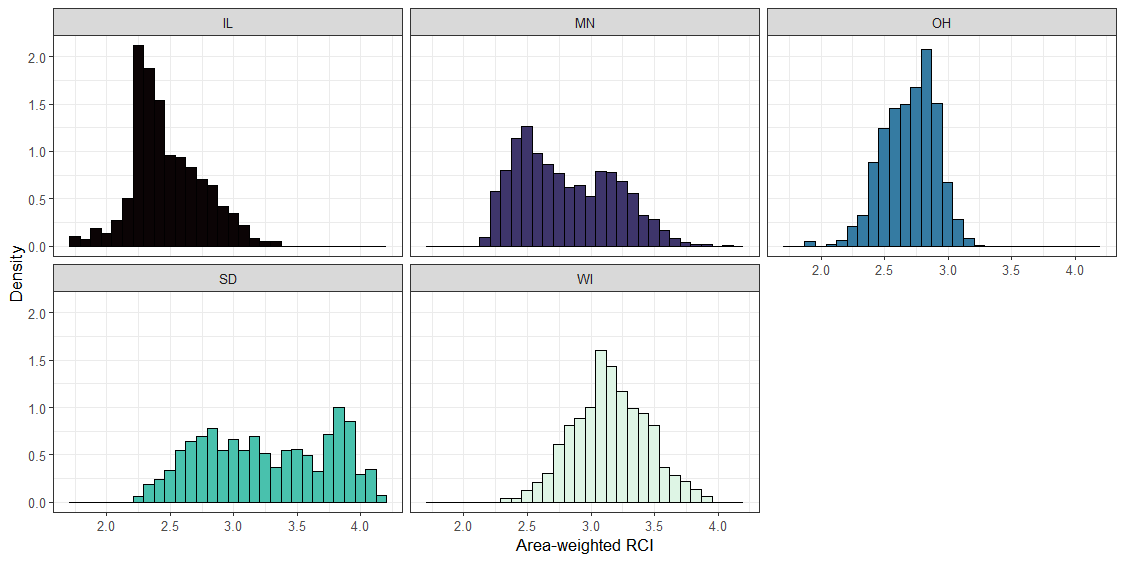
\includegraphics[scale = 0.3]{figures/rci_histograms.png}
        \caption{RCI histograms per state (2010-2020)}
        \label{fig:rci_hist} 
        \end{figure}
        \end{column}%
        \hfill%
        \begin{column}{.5\textwidth}
        \begin{figure}[H]
        \centering
        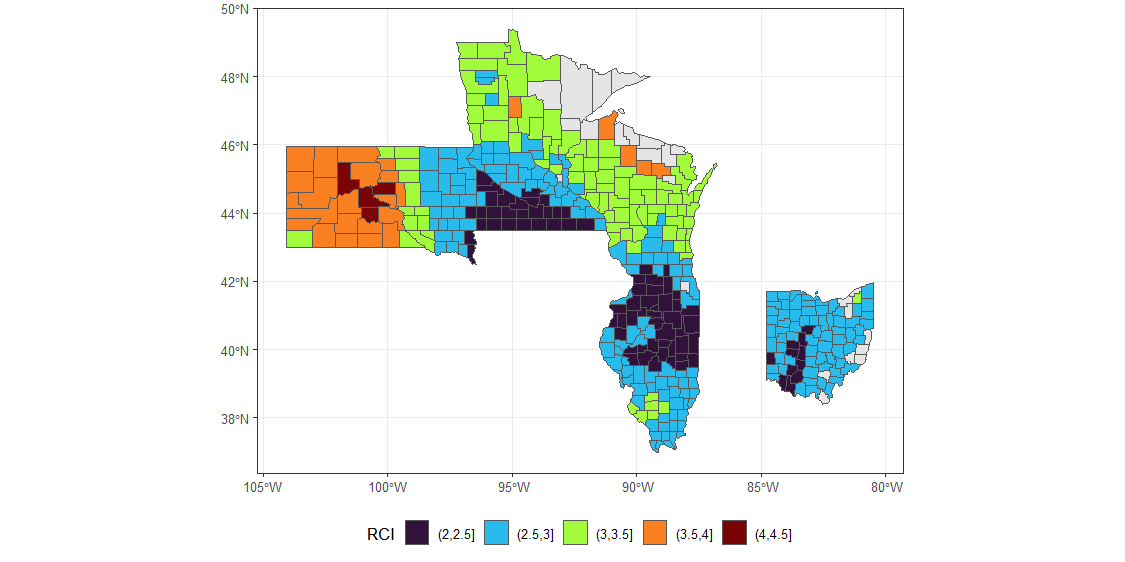
\includegraphics[scale = 0.35]{figures/rci_map.png}
        \caption{Average RCI map}
        \label{fig:rci_map} 
        \end{figure}
        \end{column}%
    \end{columns}
\end{frame}

\begin{frame}{Weather data}
    \begin{wideitemize}
        \item We use weather data from the Parameter Regression Independent Slopes Model (PRISM), following \cite{ortiz_bobea2021}.
        \item Growing Degree Days (GDD): Number of days between 8$^{\circ}$C and 29$^{\circ}$C between April and May (for preventive planting) or June-September (for pre-emergence losses) 
        \item Harmful Degree Days (HDD): Number of days above 29$^{\circ}$ between April and May (for preventive planting) or June-September (for pre-emergence losses)
        \item Average precipitation and Palmer Drought Severity Index for wet and dry conditions \citep{won2024}.
    \end{wideitemize}
\end{frame}

\begin{frame}{RCI and Loss ratios: prevented planting}
    \begin{columns}[T] % align columns
\begin{column}{.68\textwidth}
\resizebox{\textwidth}{!}{
  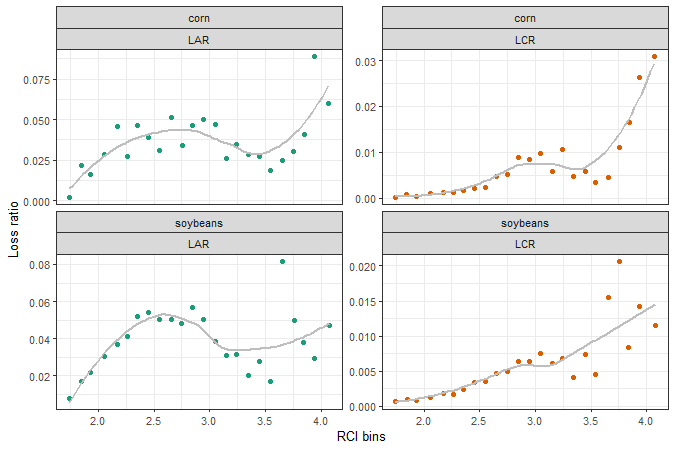
\includegraphics{figures/rci_bin_pp.png}
}
\end{column}%
\hfill%
\begin{column}{.28\textwidth}
  \begin{wideitemize}
  \item We show binned values of both loss ratios (averaged over RCI in 0.5-wide bins and RCI).
  \item Rotational complexity has a nonlinear effect on acre-based losses but less for indemnity-based losses. 
  \end{wideitemize}
\end{column}%
\end{columns}
\end{frame}

\begin{frame}{RCI and Loss ratios: post emergence}
    \begin{columns}[T] % align columns
\begin{column}{.68\textwidth}
\resizebox{\textwidth}{!}{
  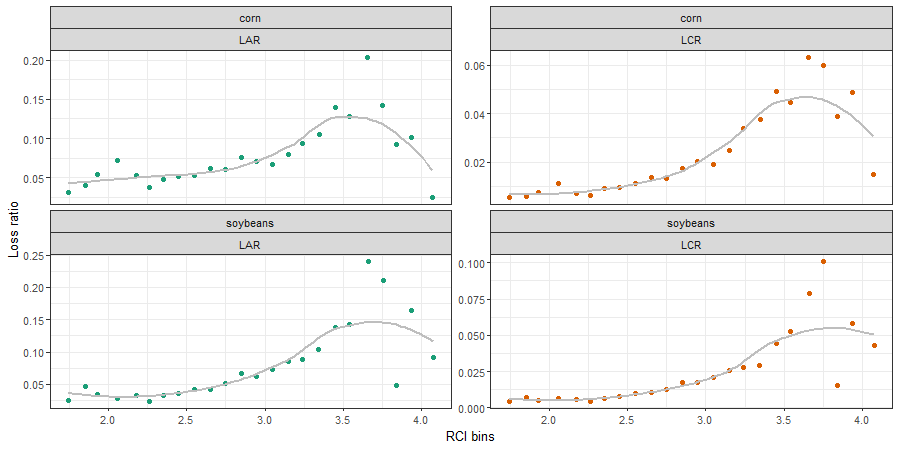
\includegraphics{figures/rci_bin_plot.png}
}
\end{column}%
\hfill%
\begin{column}{.28\textwidth}
  \begin{wideitemize}
  \item There is a slight change in the pattern.
  \item Highest losses are now observed on the top bins of rotational complexity.
  \end{wideitemize}
\end{column}%
\end{columns}
\end{frame}

%\begin{frame}{Empirical Specification: cover crop adoption}
%\begin{wideitemize}
%    \item We follow \cite{aglasan2024} and \cite{won2024}, modeling the relationship between losses ($loss_{it}$, equal to either LCR or LAR) using county-level fixed-effects, a linear time trend, and state-specific trends:

%    \begin{equation*}        loss_{it}=\beta_{cc}CC_{it}+\mathbf{W}_{it}\beta_{w}+\sum_{s}D_{s}T_{t}+\lambda T_{t}+\alpha_{i}+\varepsilon_{it}
%    \end{equation*}
%    \item $CC_{it}$: is the cover crop adoption percentage in county $i$ and year $t$, $\mathbf{W}_{it}$ are the weather variables (including a quadratic precipitation term), $T_{t}$ is the linear trend and $D_{s}$ are state-level dummies.
%\end{wideitemize}
%\end{frame}

%\begin{frame}{Cover Crop adoption (preventive planting)}
%    
\begin{table}[htbp]
   \bigskip
   \centering
   \resizebox{5.5cm}{3cm}{%
   \begin{tabular}{lcc}
      \toprule
                                  & LCR             & LAR\\  
      \midrule 
      Cover crop adoption (\%)        & -0.0169$^{***}$ & -0.0088\\   
                                  & (0.0048)        & (0.0103)\\   
      Apr-May GDD                 & -0.1449$^{***}$ & -0.3826$^{***}$\\   
                                  & (0.0166)        & (0.0333)\\   
      Apr-May HDD                 & 0.0244$^{*}$    & 0.0266\\   
                                  & (0.0147)        & (0.0216)\\   
      Apr-May PDSI wet            & -0.1709$^{***}$ & -0.9229$^{***}$\\   
                                  & (0.0603)        & (0.1257)\\   
      Apr-May PDSI dry            & 0.1894$^{***}$  & 0.4834$^{***}$\\   
                                  & (0.0706)        & (0.1449)\\   
      Apr-May Precipitation       & 0.0834$^{***}$  & 0.3403$^{***}$\\   
                                  & (0.0161)        & (0.0430)\\   
      Apr-May Precipitation$^{2}$ & -0.0011         & 0.0266\\   
                                  & (0.0307)        & (0.0868)\\   
       \\
      Observations                & 26,325          & 26,325\\  
      R$^2$                       & 0.32567         & 0.41873\\  
      Within R$^2$                & 0.02702         & 0.08497\\  
       \\
      fips fixed effects          & $\checkmark$    & $\checkmark$\\   
      year fixed effects          & $\checkmark$    & $\checkmark$\\   
      state fixed effects         & $\checkmark$    & $\checkmark$\\   
      year $\times $ state        & $\checkmark$    & $\checkmark$\\   
      \bottomrule
   \end{tabular}}
   \caption{\label{tab:fit1} Effect of cover crop adoption on losses (state-specific trends and precipitation)}
\end{table}



%\end{frame}

%\begin{frame}{Cover Crop adoption (growing period)}
%    
\begin{table}[htbp]
   \bigskip
   \centering
   \resizebox{5.5cm}{3cm}{%
   \begin{tabular}{lcc}
      \toprule
                               & LCR           & LAR\\  
      \midrule 
      Cover crop adoption      & 0.0312$^{***}$  & 0.0455$^{***}$\\   
                               & (0.0090)        & (0.0150)\\   
      May-Sep GDD              & -0.2699$^{***}$ & -0.4287$^{***}$\\   
                               & (0.0176)        & (0.0301)\\   
      May-Sep HDD              & 0.1765$^{***}$  & 0.3407$^{***}$\\   
                               & (0.0059)        & (0.0093)\\   
      May-Sep Precipitation     & -0.2658$^{***}$ & -0.5616$^{***}$\\   
                               & (0.0287)        & (0.0469)\\   
      May-Sep Precipitation sq & 0.2724$^{***}$  & 0.5069$^{***}$\\   
                               & (0.0236)        & (0.0374)\\   
      May-Sep PDSI dry         & 0.8988$^{***}$  & 2.152$^{***}$\\   
                               & (0.0735)        & (0.1567)\\   
      May-Sep PDSI wet         & -0.3375$^{***}$ & 0.3585\\   
                               & (0.1110)        & (0.2199)\\                           
       \\
      Observations             & 28,845          & 28,845\\  
      R$^2$                    & 0.46269         & 0.47891\\  
      Within R$^2$             & 0.19698         & 0.22788\\  
       \\
      fips fixed effects       & $\checkmark$    & $\checkmark$\\   
      year fixed effects       & $\checkmark$    & $\checkmark$\\   
      state fixed effects      & $\checkmark$    & $\checkmark$\\   
      year $\times $ state     & $\checkmark$    & $\checkmark$\\   
      \bottomrule
   \end{tabular}}
      \caption{\label{tab:fit2} Effect of cover crop adoption on losses (state-specific trends and precipitation)}
\end{table}



%\end{frame}

%\begin{frame}{Cover Crop adoption}
%    \begin{wideitemize}
%        \item Cover crop adoption negatively and significantly impacts the magnitude of preventive planting indemnities (LCR), but the results are reversed in the growing period.
%        \item Cover crop adoption reduces the incidence of preventive planting losses but does not have the same effect during the crop's growing period.
%        \item The positive relationship between cover crop adoption and losses is robust across several specifications.
%    \end{wideitemize}
%\end{frame}

\begin{frame}{Rotation Complexity}
\begin{wideitemize}
    \item Incorporating RCI into the model is not straightforward.
    \item RCI is bounded between 1.7 and 4.2, but its scale is not ``intuitive``, unlike cover crop percent adoption.
    \item The effect of RCI on losses is non-linear.
\end{wideitemize}
\end{frame}

\begin{frame}{Rotation Complexity}
\begin{wideitemize}
    \item We follow \cite{aglasan2024} and \cite{won2024}, modeling the relationship between losses ($loss_{it}$, equal to either LCR or LAR) using county-level fixed-effects, a linear time trend, and state-specific trends:
    \begin{equation*}        loss_{it}=f(RCI_{it})+\mathbf{W}_{it}\beta_{w}+\sum_{s}D_{s}T_{t}+\lambda T_{t}+\alpha_{i}+\varepsilon_{it}
    \end{equation*}
    \item $RCI_{it}$: is the weighted average RCI in county $i$ and year $t$, $\mathbf{W}_{it}$ are the weather variables (including a quadratic precipitation term), $T_{t}$ is the linear trend and $D_{s}$ are state-level dummies.
    \item How to model the function $f(.)$? 
    \item As categorical variable with different lengths (0.5 and 0.1); or splines as in \citep{burchfield2024}.
\end{wideitemize}
\end{frame}

\begin{frame}{RCI (preventive planting)}
    
\begin{table}[htbp]
   \bigskip
   \centering
   \resizebox{5.5cm}{3cm}{%
   \begin{tabular}{lcc}
      \toprule
                                & LCR                     & LAR\\  
      \midrule 
      rci\_cut $=$ (2,2.5]      & -0.0019                 & -0.0084\\   
                                & (0.0047)                & (0.0127)\\   
      rci\_cut $=$ (2.5,3]      & 0.0083                  & 0.0014\\   
                                & (0.0057)                & (0.0141)\\   
      rci\_cut $=$ (3,3.5]      & 0.0186$^{**}$           & 0.0316$^{*}$\\   
                                & (0.0073)                & (0.0161)\\   
      rci\_cut $=$ (3.5,4]      & 0.0290$^{**}$           & 0.0381\\   
                                & (0.0128)                & (0.0236)\\   
      rci\_cut $=$ (4,4.5]      & 0.0225                  & 0.0547\\   
                                & (0.0206)                & (0.0427)\\   
      Apr-May GDD               & -0.0002$^{***}$         & -0.0002$^{***}$\\   
                                & ($3.94\times 10^{-5}$)  & ($6.76\times 10^{-5}$)\\    
      Apr-May HDD               & 0.0009$^{***}$          & -0.0013$^{**}$\\   
                                & (0.0003)                & (0.0006)\\   
      Apr-May Precipitation     & 0.0002$^{***}$          & 0.0004$^{***}$\\   
                                & ($4.86\times 10^{-5}$)  & (0.0001)\\   
      Apr-May Precipitation\^2  & $-5.29\times 10^{-8}$   & $4.1\times 10^{-8}$\\    
                                & ($9.93\times 10^{-8}$)  & ($2.58\times 10^{-7}$)\\    
      Apr-May PDSI wet          & 0.0003                  & 0.0002\\   
                                & (0.0002)                & (0.0003)\\   
      Apr-May PDSI dry          & 0.0003$^{**}$           & 0.0005\\   
                                & (0.0001)                & (0.0003)\\   
       \\
      Observations              & 7,262                   & 7,262\\  
      R$^2$                     & 0.42314                 & 0.47086\\  
      Within R$^2$              & 0.04027                 & 0.08236\\  
       \\
      fips fixed effects        & $\checkmark$            & $\checkmark$\\   
      year fixed effects        & $\checkmark$            & $\checkmark$\\   
      state fixed effects       & $\checkmark$            & $\checkmark$\\   
      year $\times $ state      & $\checkmark$            & $\checkmark$\\   
      \bottomrule
   \end{tabular}}
      \caption{\label{tab:fit3} Effect of rotational complexity (state-specific trends and precipitation)}
\end{table}



\end{frame}

\begin{frame}{RCI (post emergence)}
    
\begin{table}[htbp]
   \bigskip
   \centering
   \resizebox{5.5cm}{3cm}{%
   \begin{tabular}{lcc}
      \toprule
                                & LCR                           & LAR\\  
      \midrule 
      rci\_cut $=$ (2,2.5]      & 0.0146$^{*}$                  & 0.0372$^{***}$\\   
                                & (0.0084)                      & (0.0136)\\   
      rci\_cut $=$ (2.5,3]      & 0.0120                        & 0.0309$^{**}$\\   
                                & (0.0091)                      & (0.0154)\\   
      rci\_cut $=$ (3,3.5]      & 0.0091                        & 0.0334$^{*}$\\   
                                & (0.0103)                      & (0.0190)\\   
      rci\_cut $=$ (3.5,4]      & -0.0071                       & -0.0180\\   
                                & (0.0139)                      & (0.0252)\\   
      rci\_cut $=$ (4,4.5]      & -0.0254                       & -0.0426\\   
                                & (0.0434)                      & (0.0988)\\   
      May-Sep GDD               & -0.0003$^{***}$               & -0.0007$^{***}$\\   
                                & ($3.66\times 10^{-5}$)        & ($6.2\times 10^{-5}$)\\    
      May-Sep HDD               & 0.0024$^{***}$                & 0.0048$^{***}$\\   
                                & (0.0001)                      & (0.0002)\\   
      May-Sep Precipitation     & -0.0004$^{***}$               & -0.0012$^{***}$\\   
                                & ($6.68\times 10^{-5}$)        & (0.0001)\\   
      May-Sep Precipitation\^2  & $4.05\times 10^{-7}$$^{***}$  & $1.11\times 10^{-6}$$^{***}$\\    
                                & ($5.53\times 10^{-8}$)        & ($1.11\times 10^{-7}$)\\    
      May-Sep PDSI wet          & $4.73\times 10^{-5}$          & 0.0020$^{***}$\\   
                                & (0.0002)                      & (0.0004)\\   
      May-Sep PDSI dry          & 0.0012$^{***}$                & 0.0032$^{***}$\\   
                                & (0.0001)                      & (0.0003)\\   
       \\
      Observations              & 7,773                         & 7,773\\  
      R$^2$                     & 0.45401                       & 0.44657\\  
      Within R$^2$              & 0.24657                       & 0.25709\\  
       \\
      fips fixed effects        & $\checkmark$                  & $\checkmark$\\   
      year fixed effects        & $\checkmark$                  & $\checkmark$\\   
      state fixed effects       & $\checkmark$                  & $\checkmark$\\   
      year $\times $ state      & $\checkmark$                  & $\checkmark$\\   
      \bottomrule
   \end{tabular}}
       \caption{\label{tab:fit4} Effect of rotational complexity (state-specific trends and precipitation)}
\end{table}



\end{frame}

\begin{frame}{RCI Coefficient plot (preventive planting)}
    \begin{figure}[H]
    \centering
    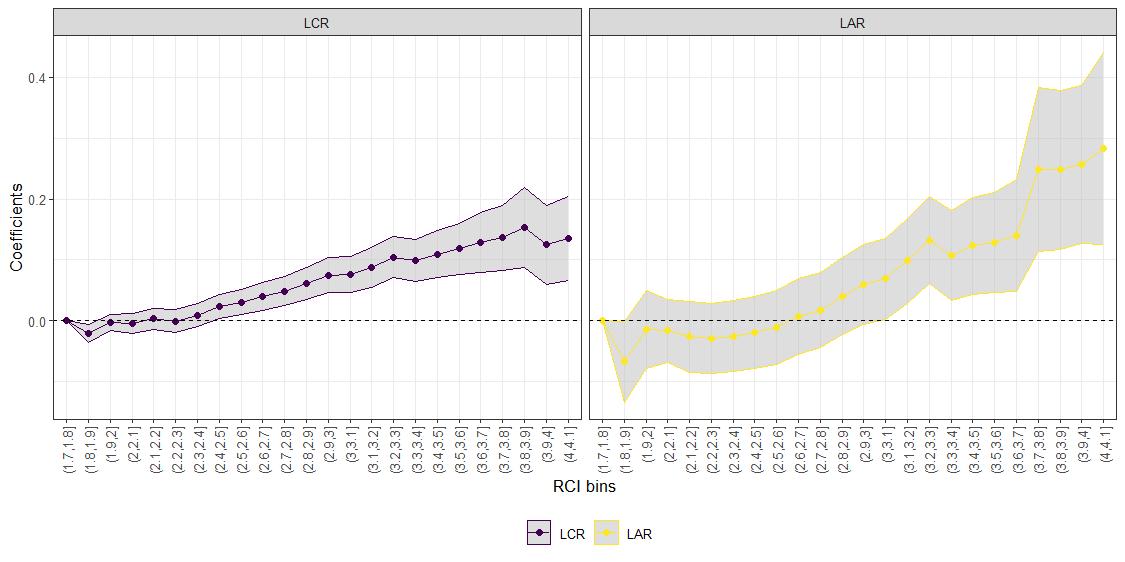
\includegraphics[scale = 0.35]{figures/coef_plot_pp.png}
    \caption{Effect of RCI on loss ratios}
    \label{fig:coef_plot_pp} 
    \end{figure}
\end{frame}

\begin{frame}{RCI Coefficient plot (post emergence)}
    \begin{figure}[H]
    \centering
    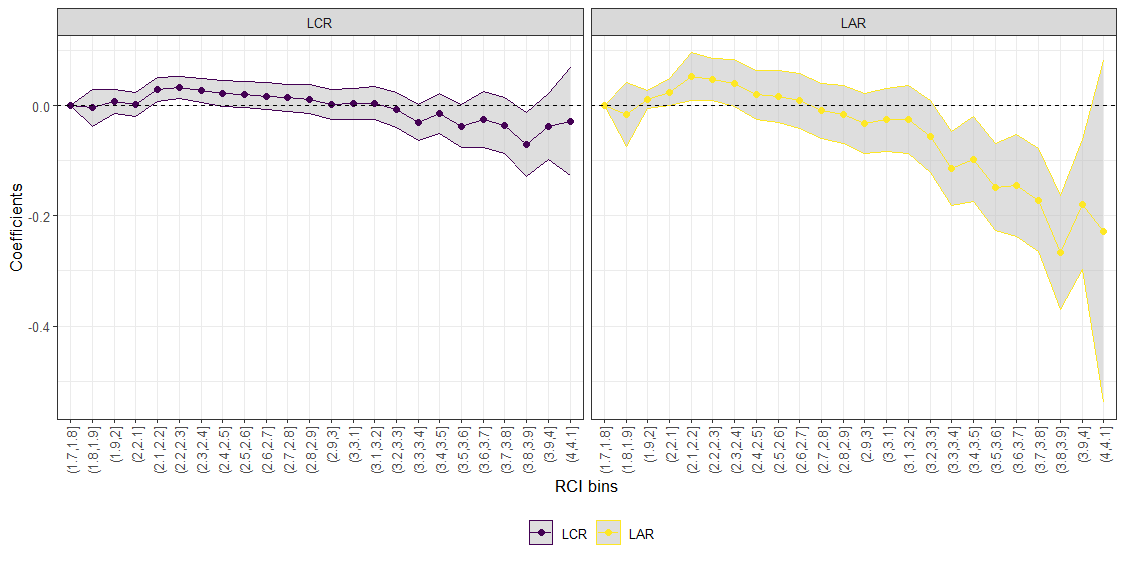
\includegraphics[scale = 0.35]{figures/coef_plot_rp.png}
    \caption{Effect of RCI on loss ratios}
    \label{fig:coef_plot_rp} 
    \end{figure}
\end{frame}

\begin{frame}{Discussion}
    \begin{wideitemize}
        \item The coefficients from the LAR model are more volatile than those of the LCR as the dependent variable.
        \item Higher RCI values led to higher preventive planting losses but lower growing season losses.
        \item Most coefficients are not significant for lower index bin values.
        \item These results appear to align with those of \cite{burchfield2024}, who find modest impacts of RCI on corn and soybean yields in a similar time frame.
    \end{wideitemize}
\end{frame}

\begin{frame}{}
	\centering \Huge
	\emph{Thank You!}
\end{frame}
	
\begin{frame}[allowframebreaks]{References}
	\bibliography{bibliography.bib}	
\end{frame}	
\end{document}
